% Created by tikzDevice version 0.12.3.1 on 2022-09-01 15:50:52
% !TEX encoding = UTF-8 Unicode
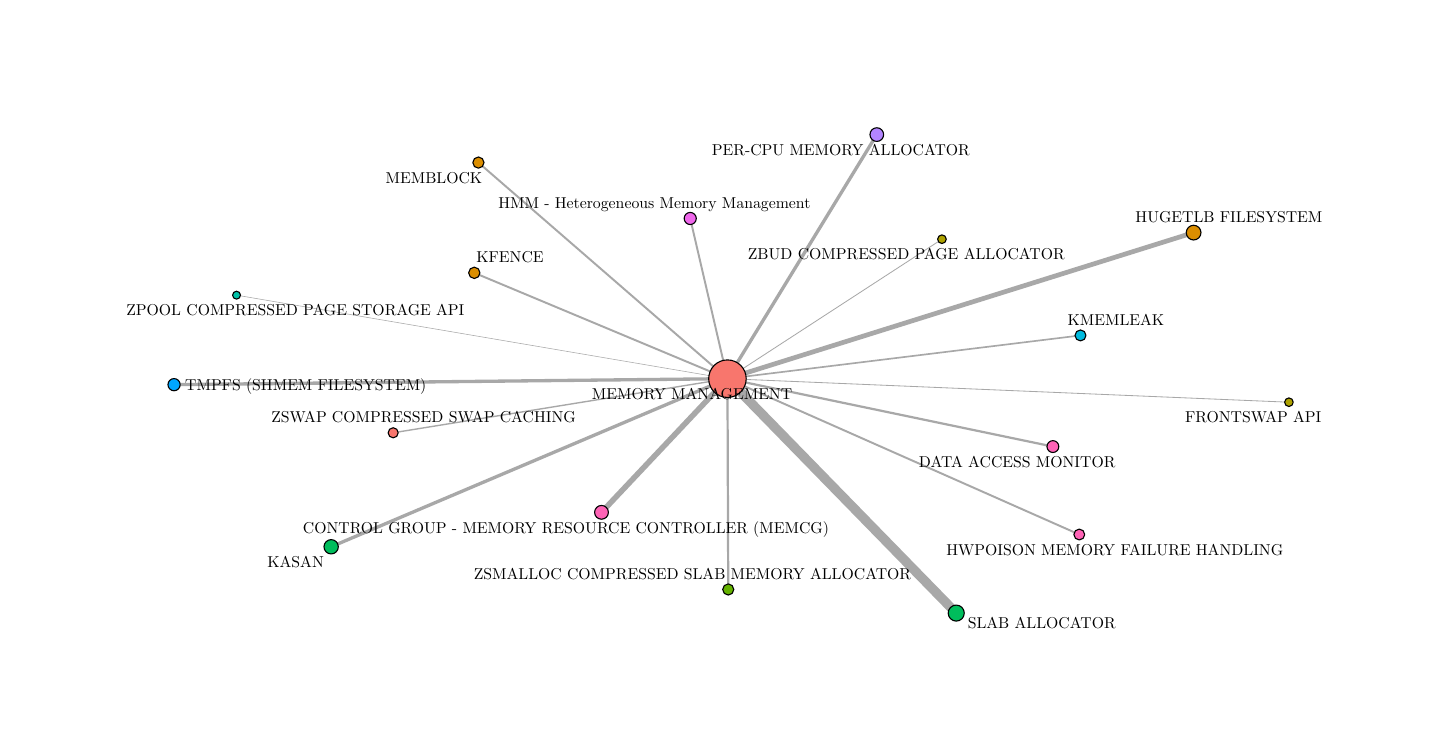
\begin{tikzpicture}[x=1pt,y=1pt]
\definecolor{fillColor}{RGB}{255,255,255}
\path[use as bounding box,fill=fillColor,fill opacity=0.00] (0,0) rectangle (505.89,252.94);
\begin{scope}
\path[clip] (  0.00,  0.00) rectangle (505.89,252.94);
\definecolor{fillColor}{RGB}{255,255,255}

\path[fill=fillColor] (  0.00,  0.00) rectangle (505.89,252.94);
\end{scope}
\begin{scope}
\path[clip] ( 32.75, 32.75) rectangle (475.89,222.94);
\definecolor{drawColor}{gray}{0.66}

\path[draw=drawColor,line width= 2.0pt,line join=round] (207.35, 77.81) -- (252.86,126.10);

\path[draw=drawColor,line width= 0.8pt,line join=round] (370.46,101.57) -- (252.86,126.10);

\path[draw=drawColor,line width= 0.3pt,line join=round] (455.75,117.60) -- (252.86,126.10);

\path[draw=drawColor,line width= 0.7pt,line join=round] (239.41,183.99) -- (252.86,126.10);

\path[draw=drawColor,line width= 1.7pt,line join=round] (421.31,178.88) -- (252.86,126.10);

\path[draw=drawColor,line width= 0.7pt,line join=round] (380.00, 69.79) -- (252.86,126.10);

\path[draw=drawColor,line width= 1.2pt,line join=round] (109.66, 65.36) -- (252.86,126.10);

\path[draw=drawColor,line width= 0.7pt,line join=round] (161.39,164.35) -- (252.86,126.10);

\path[draw=drawColor,line width= 0.6pt,line join=round] (380.43,141.73) -- (252.86,126.10);

\path[draw=drawColor,line width= 0.7pt,line join=round] (162.87,204.19) -- (252.86,126.10);

\path[draw=drawColor,line width= 1.2pt,line join=round] (252.86,126.10) -- (306.83,214.30);

\path[draw=drawColor,line width= 3.4pt,line join=round] (252.86,126.10) -- (335.53, 41.40);

\path[draw=drawColor,line width= 1.2pt,line join=round] (252.86,126.10) -- ( 52.89,123.94);

\path[draw=drawColor,line width= 0.3pt,line join=round] (252.86,126.10) -- (330.37,176.50);

\path[draw=drawColor,line width= 0.2pt,line join=round] (252.86,126.10) -- ( 75.47,156.28);

\path[draw=drawColor,line width= 0.8pt,line join=round] (252.86,126.10) -- (253.15, 49.93);

\path[draw=drawColor,line width= 0.5pt,line join=round] (252.86,126.10) -- (132.07,106.55);
\definecolor{drawColor}{RGB}{0,0,0}
\definecolor{fillColor}{RGB}{255,99,182}

\path[draw=drawColor,line width= 0.4pt,line join=round,line cap=round,fill=fillColor] (207.35, 77.81) circle (  2.49);

\path[draw=drawColor,line width= 0.4pt,line join=round,line cap=round,fill=fillColor] (370.46,101.57) circle (  2.14);
\definecolor{fillColor}{RGB}{174,162,0}

\path[draw=drawColor,line width= 0.4pt,line join=round,line cap=round,fill=fillColor] (455.75,117.60) circle (  1.55);
\definecolor{fillColor}{RGB}{239,103,235}

\path[draw=drawColor,line width= 0.4pt,line join=round,line cap=round,fill=fillColor] (239.41,183.99) circle (  2.19);
\definecolor{fillColor}{RGB}{219,142,0}

\path[draw=drawColor,line width= 0.4pt,line join=round,line cap=round,fill=fillColor] (421.31,178.88) circle (  2.66);
\definecolor{fillColor}{RGB}{255,99,182}

\path[draw=drawColor,line width= 0.4pt,line join=round,line cap=round,fill=fillColor] (380.00, 69.79) circle (  1.96);
\definecolor{fillColor}{RGB}{0,189,92}

\path[draw=drawColor,line width= 0.4pt,line join=round,line cap=round,fill=fillColor] (109.66, 65.36) circle (  2.59);
\definecolor{fillColor}{RGB}{219,142,0}

\path[draw=drawColor,line width= 0.4pt,line join=round,line cap=round,fill=fillColor] (161.39,164.35) circle (  2.05);
\definecolor{fillColor}{RGB}{0,186,222}

\path[draw=drawColor,line width= 0.4pt,line join=round,line cap=round,fill=fillColor] (380.43,141.73) circle (  1.98);
\definecolor{fillColor}{RGB}{219,142,0}

\path[draw=drawColor,line width= 0.4pt,line join=round,line cap=round,fill=fillColor] (162.87,204.19) circle (  2.02);
\definecolor{fillColor}{RGB}{248,118,109}

\path[draw=drawColor,line width= 0.4pt,line join=round,line cap=round,fill=fillColor] (252.86,126.10) circle (  6.78);
\definecolor{fillColor}{RGB}{179,133,255}

\path[draw=drawColor,line width= 0.4pt,line join=round,line cap=round,fill=fillColor] (306.83,214.30) circle (  2.47);
\definecolor{fillColor}{RGB}{0,189,92}

\path[draw=drawColor,line width= 0.4pt,line join=round,line cap=round,fill=fillColor] (335.53, 41.40) circle (  2.90);
\definecolor{fillColor}{RGB}{0,166,255}

\path[draw=drawColor,line width= 0.4pt,line join=round,line cap=round,fill=fillColor] ( 52.89,123.94) circle (  2.20);
\definecolor{fillColor}{RGB}{174,162,0}

\path[draw=drawColor,line width= 0.4pt,line join=round,line cap=round,fill=fillColor] (330.37,176.50) circle (  1.56);
\definecolor{fillColor}{RGB}{0,193,167}

\path[draw=drawColor,line width= 0.4pt,line join=round,line cap=round,fill=fillColor] ( 75.47,156.28) circle (  1.43);
\definecolor{fillColor}{RGB}{100,178,0}

\path[draw=drawColor,line width= 0.4pt,line join=round,line cap=round,fill=fillColor] (253.15, 49.93) circle (  2.01);
\definecolor{fillColor}{RGB}{248,118,109}

\path[draw=drawColor,line width= 0.4pt,line join=round,line cap=round,fill=fillColor] (132.07,106.55) circle (  1.82);

\node[text=drawColor,anchor=base,inner sep=0pt, outer sep=0pt, scale=  0.57] at (194.49, 70.32) {CONTROL GROUP - MEMORY RESOURCE CONTROLLER (MEMCG)};

\node[text=drawColor,anchor=base,inner sep=0pt, outer sep=0pt, scale=  0.57] at (357.57, 94.07) {DATA ACCESS MONITOR};

\node[text=drawColor,anchor=base,inner sep=0pt, outer sep=0pt, scale=  0.57] at (442.85,110.10) {FRONTSWAP API};

\node[text=drawColor,anchor=base,inner sep=0pt, outer sep=0pt, scale=  0.57] at (226.45,187.57) {HMM - Heterogeneous Memory Management};

\node[text=drawColor,anchor=base,inner sep=0pt, outer sep=0pt, scale=  0.57] at (434.08,182.42) {HUGETLB FILESYSTEM};

\node[text=drawColor,anchor=base,inner sep=0pt, outer sep=0pt, scale=  0.57] at (392.82, 62.32) {HWPOISON MEMORY FAILURE HANDLING};

\node[text=drawColor,anchor=base,inner sep=0pt, outer sep=0pt, scale=  0.57] at ( 96.83, 57.87) {KASAN};

\node[text=drawColor,anchor=base,inner sep=0pt, outer sep=0pt, scale=  0.57] at (174.30,167.95) {KFENCE};

\node[text=drawColor,anchor=base,inner sep=0pt, outer sep=0pt, scale=  0.57] at (393.24,145.28) {KMEMLEAK};

\node[text=drawColor,anchor=base,inner sep=0pt, outer sep=0pt, scale=  0.57] at (146.80,196.69) {MEMBLOCK};

\node[text=drawColor,anchor=base,inner sep=0pt, outer sep=0pt, scale=  0.57] at (240.07,118.62) {MEMORY MANAGEMENT};

\node[text=drawColor,anchor=base,inner sep=0pt, outer sep=0pt, scale=  0.57] at (293.86,206.79) {PER-CPU MEMORY ALLOCATOR};

\node[text=drawColor,anchor=base,inner sep=0pt, outer sep=0pt, scale=  0.57] at (366.43, 35.76) {SLAB ALLOCATOR};

\node[text=drawColor,anchor=base,inner sep=0pt, outer sep=0pt, scale=  0.57] at (100.49,121.99) {TMPFS (SHMEM FILESYSTEM)};

\node[text=drawColor,anchor=base,inner sep=0pt, outer sep=0pt, scale=  0.57] at (317.49,169.01) {ZBUD COMPRESSED PAGE ALLOCATOR};

\node[text=drawColor,anchor=base,inner sep=0pt, outer sep=0pt, scale=  0.57] at ( 96.73,148.81) {ZPOOL COMPRESSED PAGE STORAGE API};

\node[text=drawColor,anchor=base,inner sep=0pt, outer sep=0pt, scale=  0.57] at (240.20, 53.49) {ZSMALLOC COMPRESSED SLAB MEMORY ALLOCATOR};

\node[text=drawColor,anchor=base,inner sep=0pt, outer sep=0pt, scale=  0.57] at (143.04,110.13) {ZSWAP COMPRESSED SWAP CACHING};
\end{scope}
\end{tikzpicture}
